\section{\mc 背景}
約1世紀前にHans Bergerによって世界で初のヒトの脳活動計測の試みがなされた\cite{宮内1,宮内2,宮内3}。
以降、脳活動を計測するための測定装置が開発され、
特に近年は以下の応用を目指した脳信号の解析と解読に大きな関心が寄せられている。
\begin{itemize}
    \item 医療応用:脳信号は、認知症やてんかん発作のような様々な精神障害の診断、
    および治療のために活用されている\cite{精神疾患,認知症}。
    \item 生体認証:脳信号は偽造、盗聴が困難であることから、
    固体の識別のための普遍的な生体情報となりうる\cite{個人認証,ウェアラブル個人認証}。
    \item Brain Computer Interface(BCI):
    BCIは``direct neural interface''や``brain machine interface''とも表現され、
    外界と筋肉の動作無しに相互作用するためのインターフェースの役割を担う\cite{DNI}。
    初期のBCIは麻痺患者や障害のある患者の
    生活補助装置を制御するように設計された\cite{BCIbasic}。
    更に、近年は高度な精神的タスクを実行する健常者の支援や
    仮想空間での入力装置としての商用BCIが登場するに至っている\cite{VRBCI,VRBCIsv}。
\end{itemize}
BCIにおいて脳信号を計測する方法は、大きく分けて以下の3つがある。
\begin{itemize}
    \item 侵襲式:脳へセンサを直接埋め込む方式
    \item 部分侵襲式:頭蓋骨の内部、脳の表面へセンサを埋め込む方式
    \item 非侵襲式:センサを頭蓋骨外部へ配置し、外科手術を必要としない方式
\end{itemize}
侵襲式BCIの利用範囲は安全に配慮して臨床試験に限られている。
対照的に、非侵襲式は外科手術の必要性がなく、
商業及び医療的な用途の両方に用いられており、今後更に発展する可能性があるため
本研究では非侵襲式の計測方法に着目する。

BCIで用いられる非侵襲式の計測には以下のようなものがある。
\begin{itemize}
    \item functional Magnetic Resonance Imaging (fMRI):
    MRIによって脳活動時の血流によって生ずる磁場を測定する。
    この測定は、脳の神経細胞が活動中により多くの酸素を含む血流を必要とする
    という事実に基づいている。
    \item functional Near-Infrared Spectroscopy (fNIR):
    近赤外線電磁波を用いて、
    脳皮質の異なる部分における酸素化および脱酸素化ヘモグロビンの濃度を測定する。
    \item Magnetoencephalography (MEG):
    この方法は、高感度磁力計アレイを使用して、
    脳の神経活動によって生成される磁場を直接測定する。
    MEGを利用する大きな利点は、
    頭蓋骨や他の組織は磁場に対してほとんど透明であるため、
    減衰や歪みが生じないことが挙げられる。
    \item Electroencephalography (EEG):
    この方法では頭皮上にいくつかの小さな電極を配置し、
    脳全体の神経アセンブリによって生成された電場を測定する。
\end{itemize}
これらの方法の中で、fMRIおよびMEGは、fNIRおよびEEGと比較して比較的高い空間分解能を提供する\cite{脳を測る}。
しかし、fMRI(図\ref{fig:fMRI})及びMEG(図\ref{fig:MEG})
は非常に高価な装置である上に大型機器であるため、
BCIアプリケーションで必要とされるような要件を満たすとは言い難い。
一方でfNIRはポータブルであるが、
脳活動から数秒程度の遅れで測定が行われるという欠点を有する\cite{脳を測る}。
\begin{figure}
    \begin{center}
    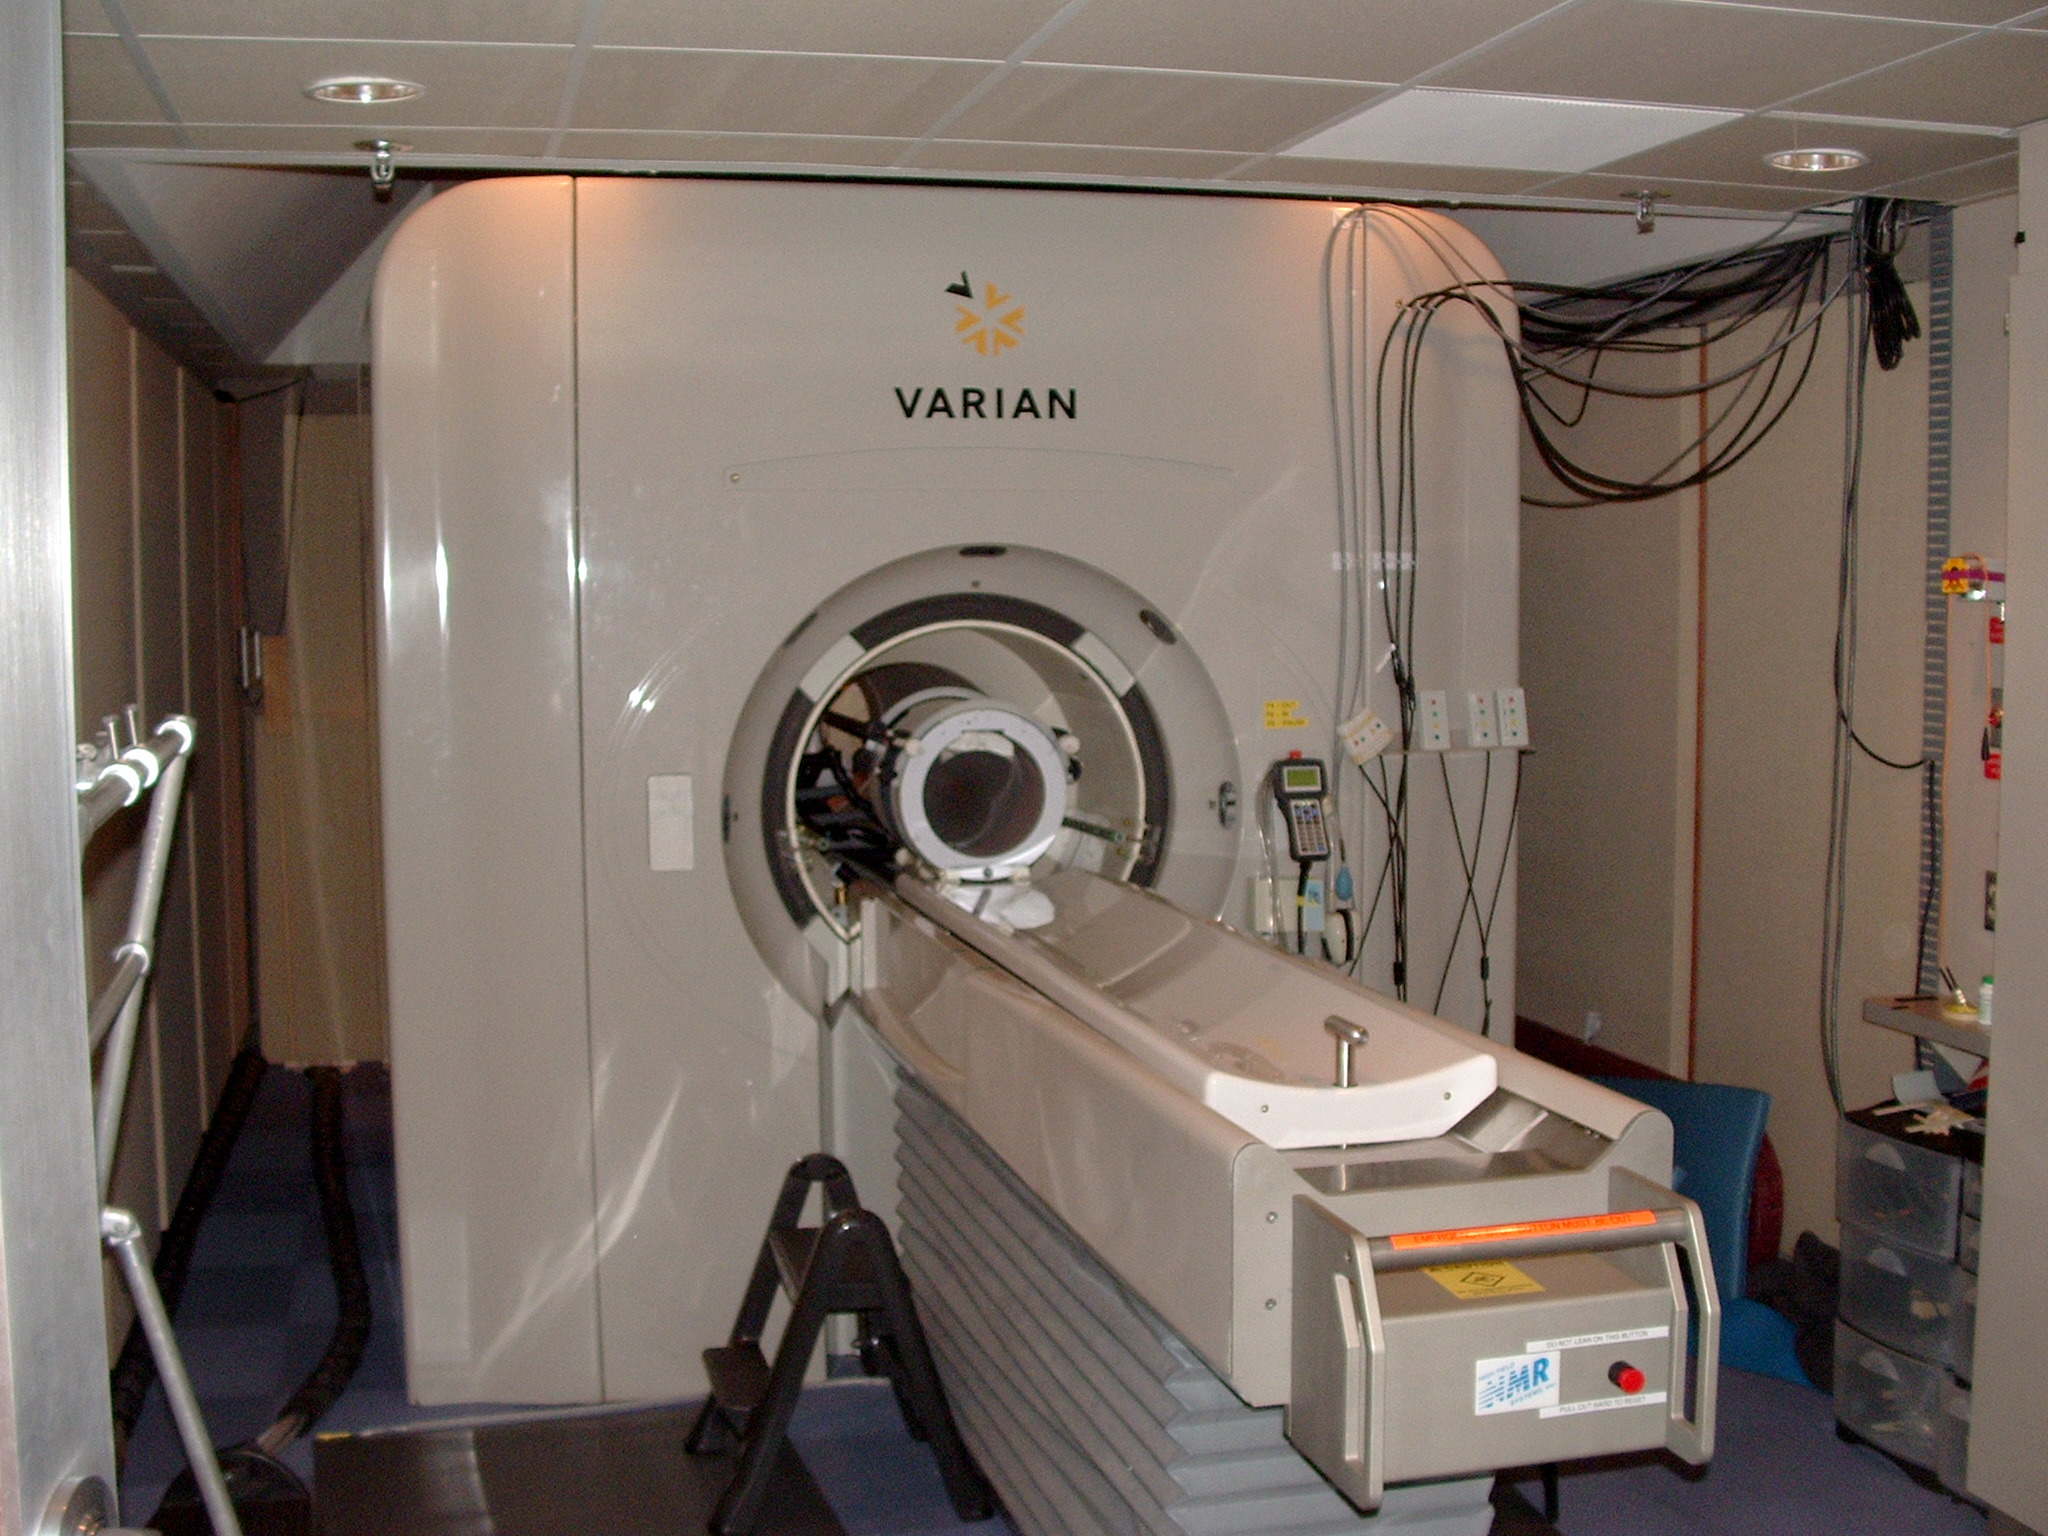
\includegraphics[width=120mm]{images/fMRI.jpg}
    \end{center}
    \caption{fMRI}
    \label{fig:fMRI}
\end{figure}
\begin{figure}
    \begin{center}
    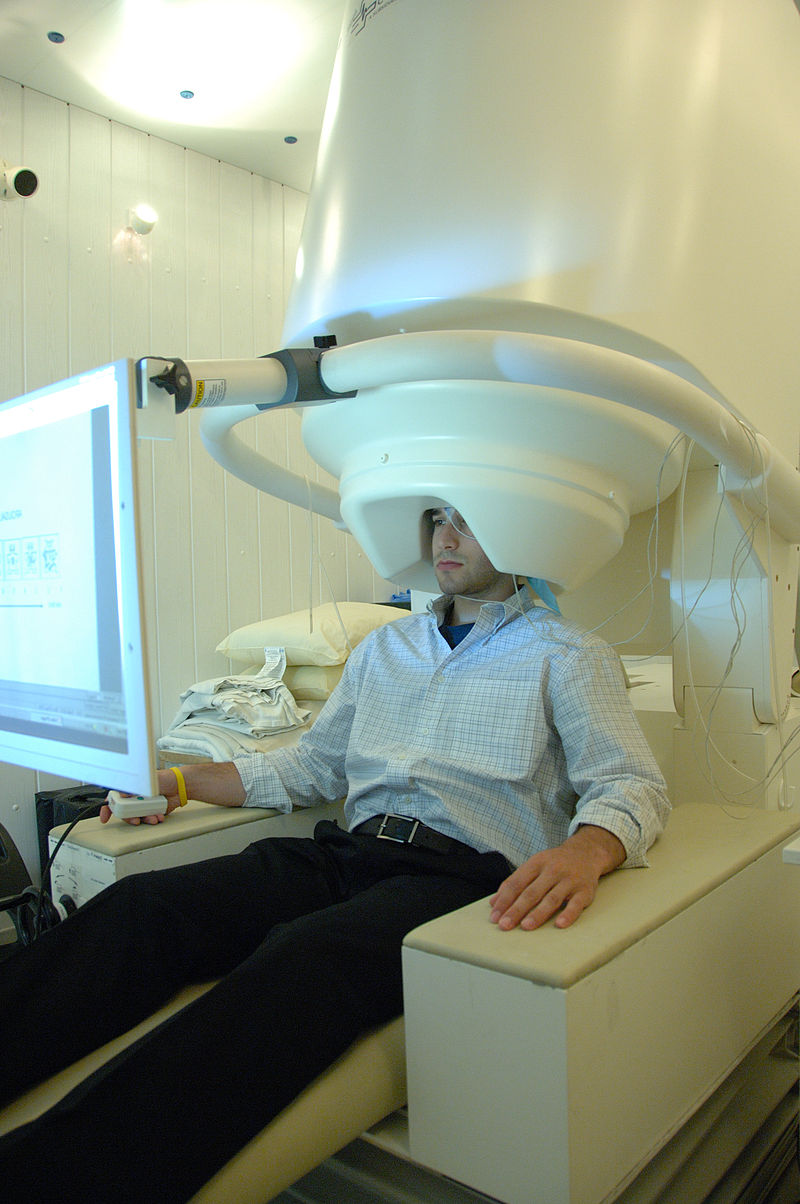
\includegraphics[width=70mm]{images/MEG.jpg}
    \end{center}
    \caption{MEG}
    \label{fig:MEG}
\end{figure}

\begin{figure}
    \begin{center}
    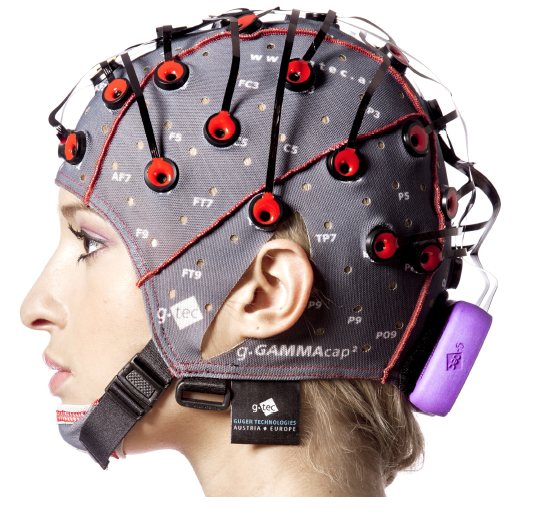
\includegraphics[width=60mm]{images/eeg.png}
    \end{center}
    \caption{EEGキャップ(ミユキ技研)}
    \label{fig:EEG}
\end{figure}
% \begin{figure}[t]
%     \begin{minipage}{0.5\hsize}
%         \begin{center}
%             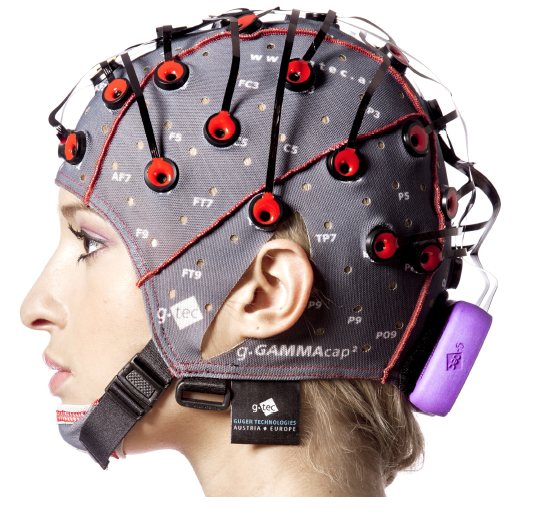
\includegraphics[width=60mm]{images/eeg.png}
%         \end{center}
%         \caption{fNIRキャップ(参照明記englishwiki)}
%         \label{fig:fNIR}
%     \end{minipage}
%     \begin{minipage}{0.5\hsize}
%         \begin{center}
%             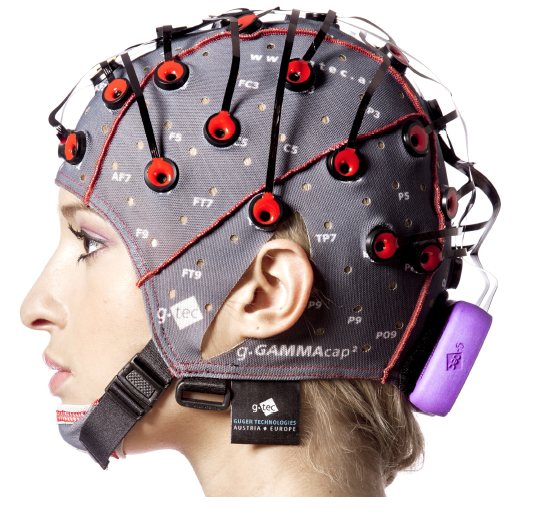
\includegraphics[width=60mm]{images/eeg.png}
%         \end{center}
%         \caption{EEGキャップ(ミユキ技研)}
%         \label{fig:EEG}
%     \end{minipage}
% \end{figure}

宮内氏の技術報告書\cite{脳を測る}によると、
EEGによる脳活動の計測に関して以下の記述がある(一部改変)。
\begin{quotation}
ヒトの脳活動計測によって獲得したいものは、精神活動・行動の生物学的基盤となる
脳の神経細胞(ニューロン)の電気的活動だが、
個々のニューロンの活動を非侵襲的に計測する事は不可能である。
しかし、ニューロンの活動に伴って様々な生理現象が生ずる。
まずニューロンが電気的な活動(一次信号)を行うためにはエネルギーを必要とし、
糖の分解のための代謝活動(二次信号)が生ずる。
酸素と糖は脳にはほとんど貯蔵されていないため、
代謝活動に伴ってエネルギーを必要としている脳の部位に関して、局所脳血流(三次信号)が増大する。
EEGやMEGは脳の電気的な活動である一次信号を計測しており、
fMRIやNIRSは血流に関する三次信号を計測している(図\ref{fig:信号フロー}\cite{脳を測る})。
\end{quotation}
\begin{figure}
    \centering
    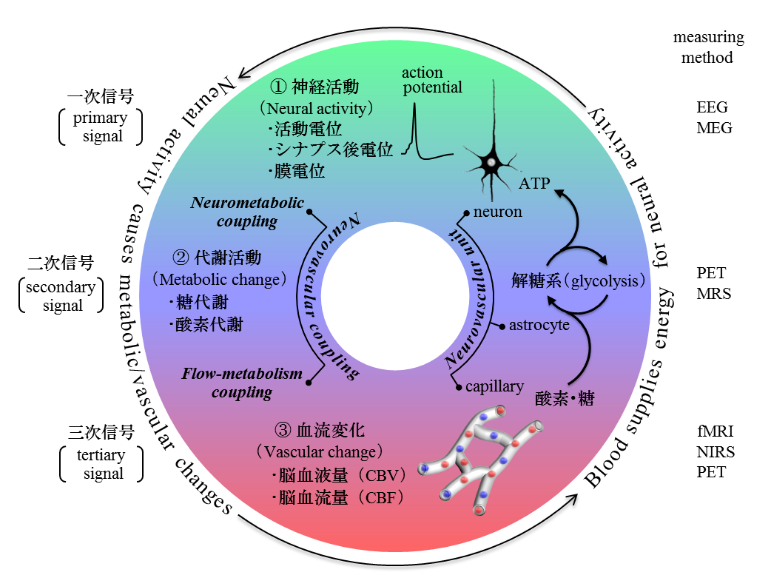
\includegraphics[width=12cm]{images/signalflow.png}
    \caption{一次信号、二次信号、三次信号と計測方法の関係図\cite{脳を測る}}
    \label{fig:信号フロー}
\end{figure}
EEGは一次信号を計測したものであり
NIRSやfMRIに比べ脳活動に対する測定値の遅れは少ないことが利点となる。
この利点に加え、EEGの測定装置は比較的安価であるため本研究の焦点とする。

続いて同様に\cite{脳を測る}にはEEGの分解能に関して以下の記述がある。
\begin{quotation}
また非侵襲計測の中では最も時間分解能が高いとされる。
ここで時間分解能とは脳の同一の場所が短時間に二回活動した場合に、
それぞれを時間的に独立した脳活動として計測できる最短の時間間隔である。
一方で頭蓋骨や皮膚、毛髪などは電位にとっては透明ではないため空間分解能は低いとされる。
ここで空間分解能とは脳の異なる部位が同時に二箇所活動した場合に、それぞれを活動部位が異なる
独立した脳活動として計測できる最小の距離である。
ただし、通常の計測においては計測装置の空間分解能や時間分解能は測定対象には依存しないが、
脳活動計測の場合においては一般的に計測対象としている現象の時空間特性や脳活動の強さ、
あるいは発生源が皮膚表面であるか脳の深部であるかなどにも依存する。
\end{quotation}
時間分解能の高さはBCIをEEGに基づいて動作させる利点となるが、
空間分解能の低さは明らかな欠点となるため、何らかの対策が必要となる。

\section{{\rm EEG}\mc に基づく{\rm BCI}{\mc の概要}}
\subsubsection{\rm BCI\mc の動作原理}
BCIの動作は以下のスキームに従う。
\begin{enumerate}
    \item 脳信号の獲得:センサによりアナログ信号を獲得しディジタル信号へ変換
    \item 信号の前処理:データの成形及びアーチファクトの除去
    \item 特徴量抽出:神経科学や統計に基づいた特徴量の選定
    \item 分類:特徴量から閾値に基づいて意図を分類
    \item 制御信号出力:分類結果に基づいて外部機器へ信号を出力
\end{enumerate}
BCIの種類に関わらず動作原理の根本は同様であるが、
スキームのどの段階に課題が生じるかは異なると考えられる。
侵襲式の場合は脳信号の獲得自体が困難であり、安全性やメンテナンス性に課題が生ずる。
非侵襲式の場合は脳信号の獲得は気軽に実施できるが、空間分解能や時間分解能の問題、
あるいはアーチファクトの存在によって意図を復元することは容易ではないと推察される。
従ってEEGを用いた運動想起型BCIに焦点を当てる場合、主に特徴量抽出と分類の段階が課題となる(図\ref{fig:BCIsystem})。

\begin{figure}[tb]
    \centering
    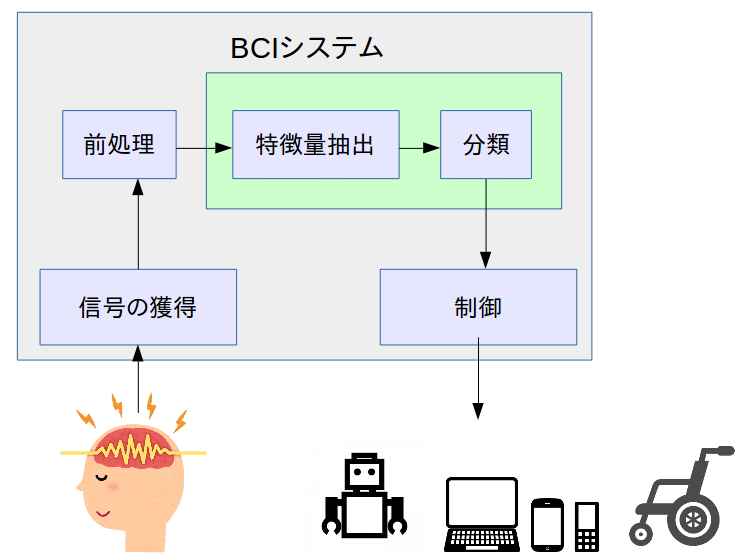
\includegraphics[width=13cm]{images/BCIsystem.png}
    \caption{BCIの動作スキーム}
    \label{fig:BCIsystem}
\end{figure}

またEEGに基づくBCIシステムに関しても、
着目するEEGの種類に応じて以下の二種に大別することができる。
\subsubsection{{\mc 誘発型}\rm BCI}
外部刺激によって誘発されるタイプのBCIを本論文では誘発型BCIとまとめて表記する。
例として、ユーザがBCIシステムを使用してマウスカーソルを動作させたいとする。 
この時、異なる周波数で点滅する複数の光源をユーザに提示することで、
注視した光源に応じた誘発電位を生成させることができる\cite{SSVEP}。
結果として、光源を見たユーザの脳信号を分析することでマウスカーソルの動作方向を決定することが可能である。
このタイプのBCIは通常、SSVEP型BCIと呼ばれる。

誘発電位を用いたBCIシステムは非常に正確であるが、
ユーザは常に刺激に直面するため、長期的な使用には向いていない。
また、BCIシステム自体が刺激装置などの外部機器を必要とする。
\subsubsection{\mc 自発型 \rm BCI}
一方で外部刺激に依らないEEGを用いて動作するBCIを自発型BCIと呼ぶ。
自発型BCIの中でも特に、特定の身体部位の動作を想像することで動作する運動想起型BCIに注目する。
運動想起型BCIの簡単な例を示すために、ユーザがBCIシステムを使用してマウスカーソルを動作させる例を見る。
この時、マウスカーソルを左に動かしたい場合は左手の運動を想起し、マウスカーソルを右に動かしたい場合は右手の運動を想起する。
また、下に動かしたい場合は左足、上に動かしたい場合は右足、
というように想起する身体部位に応じて外部機器への制御信号を対応させることが可能である。
同様の応用方法が車いすなどにも適用できる。

運動想起型BCIを使う利点の1つは、運動想起によって生成されたEEG信号は、
物体の想像、あるいは抽象的な概念を想像する他の精神的イメージのタスクと比較して一貫性がある点である。
一般に、運動想起によって活性化される神経は、運動を実際に実行する場合と同様であるとされる\cite{運動想起}。
本研究では運動想起型BCIに焦点を当てる。
これまでのBCIの分類について図\ref{fig:BCIclass}に示す。

\begin{figure}[tb]
    \centering
    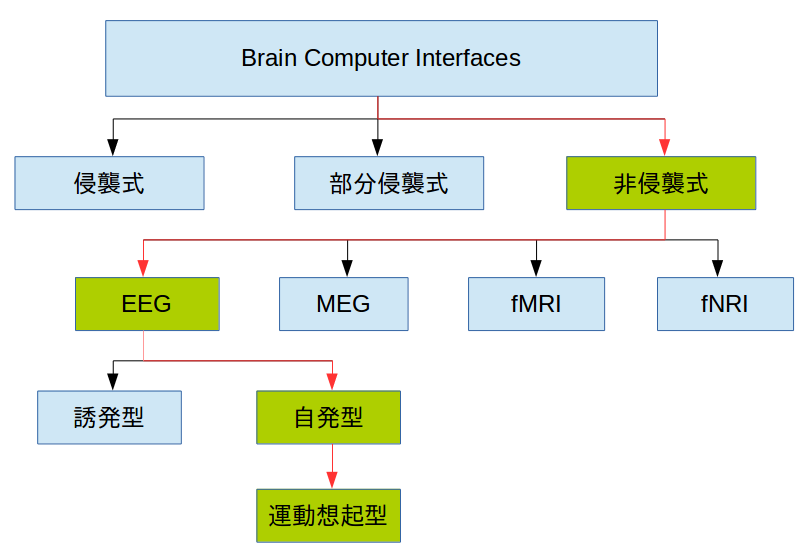
\includegraphics[width=13cm]{images/BCIclass.png}
    \caption{BCIの分類と本研究の焦点}
    \label{fig:BCIclass}
\end{figure}


\subsubsection{\mc 運動想起型\rm BCI\mc 周辺の研究}
運動想起時には運動野付近で特定の周波数帯域において活動電位が減少する
事象関連脱同期(Event Related Desynchronization : ERD)の存在が知られており、
神経科学的な、あるいはBCI応用のための研究が盛んに行われている\cite{ERDとERS,ERDリハビリ,運動フィードバック}。
従って特徴量としてERDが用いられる研究も数多くあり、EEGを用いた運動想起型BCIでも基礎となっている\cite{プリミティブERD,Beta波によるBCI,waveletFSVM}。
ERDを発見することができた場合、EEGの振幅あるいはパワーに閾値を設けて分類を行うことができる。
具体的にはスペクトル解析によって各周波数のパワーを推定し、パワーに閾値を設けることとなる。
しかし、EEGからのERDの検知は必ずしも容易ではない。
ERDが生じる頭皮上の位置と周波数は個人差がある上、
有効な周波数スペクトル解析に関しても未だ研究段階である\cite{時間周波数解析の比較}。

また、人の随意運動の約0.5秒から1秒前に現れる運動準備電位も特徴量になると考えられている。
実動作以前に発生するという極めて特殊な現象であるため、
その特性からBCIが人の意志に対して優れた反応速度で動作することが期待される。
BCIの研究としては実肢体動作の分類\cite{運動準備電位肢体}や実指動作の分類\cite{運動準備電位指}などがある。
実運動を行わなくとも運動準備電位が特徴量として活用できるという研究\cite{運動準備電位想起,運動準備電位想起2}もある。

一方で特定のEEGの現象を直接獲得せずに運動想起型BCIを構築する手法も提案されており、
それらの多くが統計的信号処理や機械学習を活用したものである。
特にCommon Spatial Pattern(CSP)と呼ばれる統計的信号処理\cite{CSP1990,CSP1999}は、
EEG解析のために発案されて以降、現在までに様々な派生手法を生み出している\cite{csssp,正則化CSP,カーネルCSP,cvscsp}。
その中でもFilter Bank Common Spartial Pattern\cite{fbcsp}と呼ばれるCSPの
発展手法は、ERDに基づくBCIも含め他の手法と比べ高い性能を有している。

現在、EEGの現象として知られている既知の特徴量を検知する手法から、
機械学習や統計的信号処理を活用した特徴量抽出手法と高度な分類器を組み合わせ
高い性能を発揮する手法の模索が行われている\cite{BCIの比較}。
